\documentclass[10pt, a4paper]{article}

\usepackage[frenchb]{babel}
\usepackage[T1]{fontenc}
\usepackage[left=2.2cm, right=2.2cm, top=2.5cm, bottom=2.5cm]{geometry} % Mise en page
\usepackage{tikz}
\usepackage{lscape}
\usepackage{graphicx}

\author{Florian \bsc{Thuin} (06561100) \and Gregory \bsc{Vander Schueren}}
\title{LINGI1131 - Oz Project Report}
\date{\today}

\begin{document}

\maketitle

\section{Data structures}

We use the following 4 main data structures (implemented with records) across the project:

\begin{description}
  \item [GameState:] The GameState is the top level data structure. It holds all the information describing the current state of the game. It is passed around by the gameLoop and modified at each turn. It holds the following information: turn(number), player, trainers(list) and map\_info.
  \item [MapInfo:] Holds the map record and various information like: victory\_position, hospital\_position and width/height for convenience.
  \item [Player:] The player structure describes the player or an enemy trainer. It hold the following info: name, image, position, selected\_pokemoz and pokemoz\_list.
  \item [Pokemoz:] The pokemoz structure describes any pokemoz: name, type, level, health and xp.

\end{description}

\section{Components}

Our project is separated into 12 functors or \og{}components\fg{}. This sections describe the role of each of those components and how they interact together:

\begin{enumerate}
  \item Main components
    \begin{description}
     \item[Game:] The Game component is the main program which is run when you start the game. It's main responsibilities are: getting the program parameters, setting up the main window and receiving keyboard inputs, setting up the intial game state, launching and managing the gameloop. Aside from that it mostly relies on the other components to do all the heavy lifting.
     \item[Fight:] Manage the fight between trainers or trainer VS wild pokemoz.
     \item[AutoPilot:] Manage the autoplay if this option is given in command line by exposing only one function (GenerateNextInstruction) to the game component.
    \end{description}
  \item User interface components
    \begin{description}
     \item[Intro:] Responsible for drawing and managing an interface that allows the player to enter his name and choose his starting pokemoz. It exposes only one function (GetUserChoice) to the game component.
     \item[Map:] Responsible for drawing and managing the map section of the interface. It exposes multiple functions to set items positions and animates items (ie. DrawPlayer or MovePlayer).
     \item[Interface:] Responsible for drawing and managing the lower interface. It exposes multiples functions for displaying the game state (ie. UpdatePlayer1) or getting user input (ie. AskQuestion).
    \end{description}
  \item Helper components
    \begin{description}
     \item[Characters:] Define the game characters (all the pokemoz and trainers).
     \item[Strings:] Define all the text strings displayed in the multiple interfaces.
     \item[Lib:] Exposes general purpose functions.
     \item[GameState:] Helpers to mutate and read data from a gameState record.
     \item[Player:] Helpers to mutate and read data from a player record.
     \item[Pokemoz:] Helpers to mutate and read data from a pokemoz record.
    \end{description}
\end{enumerate}




\begin{landscape}

\begin{figure}

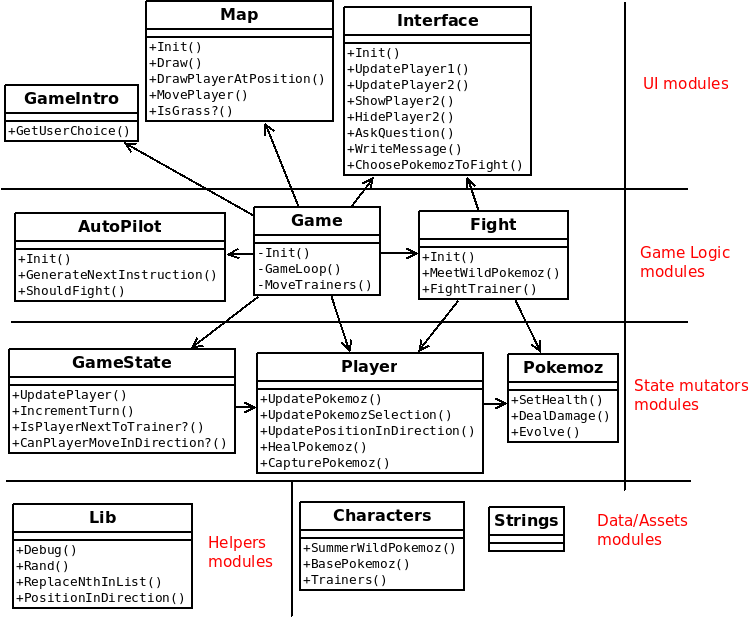
\includegraphics[width=\linewidth]{Diagramme1.png}
\caption{Component diagram of our project}
\end{figure}

\end{landscape}


\section{State diagrams}

\begin{figure}[!ht]
 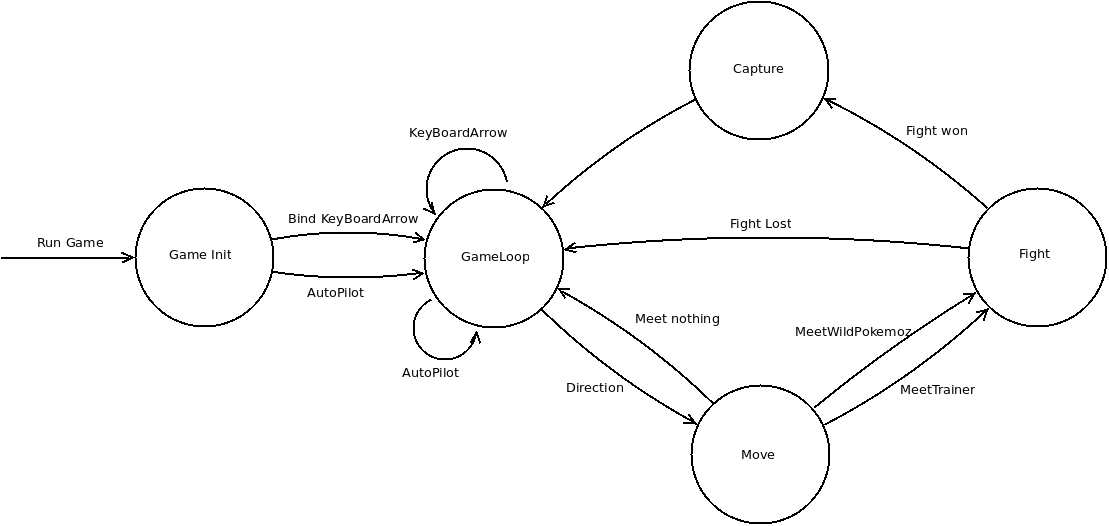
\includegraphics[width=\linewidth]{State_diagram_oz.png}
 \caption{State diagram of our project}
\end{figure}


\end{document}
